
\chapter{Grover's algorithm} \label{GA_theo}
In previous chapter we defined all necessary requirements for describing one of the most known quantum algorithms described by L. K. Grover \cite{grover1996fast}. It is a probabilistic algorithm, where we iterate the right gates the right amount of times to obtain the highest probability of measuring the correct result; this means that we have to run the algorithm multiple times as incorrect solution may occur, or if we have multiple correct results, we need to measure it multiple times so that all correct results are measured.

The problem is defined as follows, say we have $N$ items in a database and we would like to find one or more with desired properties. 

The difference between the classical and the quantum versions of the algorithm is in the number of steps we have to take. For this, it is a good idea to introduce the definition of the $O$ notation.

We are given functions $f(n): {\rm I\!N} \rightarrow {\rm I\!R}, g(n): {\rm I\!N} \rightarrow {\rm I\!R}$. 
\newline
We say, that $f(n) \in O(g(n))$, if $ (\exists n_o \in {\rm I\!N})(\exists c \in {\rm I\!R})(\forall n \in {\rm I\!N} : n > n_0) : f(n) \le cg(n)$. We can understand the function $g$ as some kind of upper bound for the function $f$.

According to our definition, the classical algorithm would require $O(N)$ to find all solutions to the problem. For the quantum algorithm, it takes just $O(\sqrt{N})$. Our database has $2^n$ items in it, because there are exactly $2^n$ combinations of ones and zeros for n bits. This means that the classical algorithm runs with a time complexity of $O(2^n)$, but quantum only with a complexity of $O(\sqrt{2^n}) = O(2^{\frac{n}{2}})$, which is a significant improvement.

\section{Algorithm workflow} \label{Algorithm_workflow}
In this section we will visualise and describe the concept of the algorithm. In the next chapters we will describe it more analytically and give more in-debt explanation.
\subsection{State preparation}
The algorithm itself has three parts. Say, we have $n$ qubits for our database, $m$ ancilla qubits, which can be scraped, and one qubit on top of that. Note that we will focus only on states of $n$ qubits, which holds our information on our computation, and we will not focus on ancilla and extra qubits.

In the first step, preparation, we will set the n qubits in such a state that the probability of measuring any of $2^n$ is uniform. This is done by using the Hadamard gate on them. In the same step we set the extra qubit in $|-\rangle$, which is done by using the Hadamard gate followed by the X gate. This leaves us with the following:

\begin{center}
\begin{figure}[h]
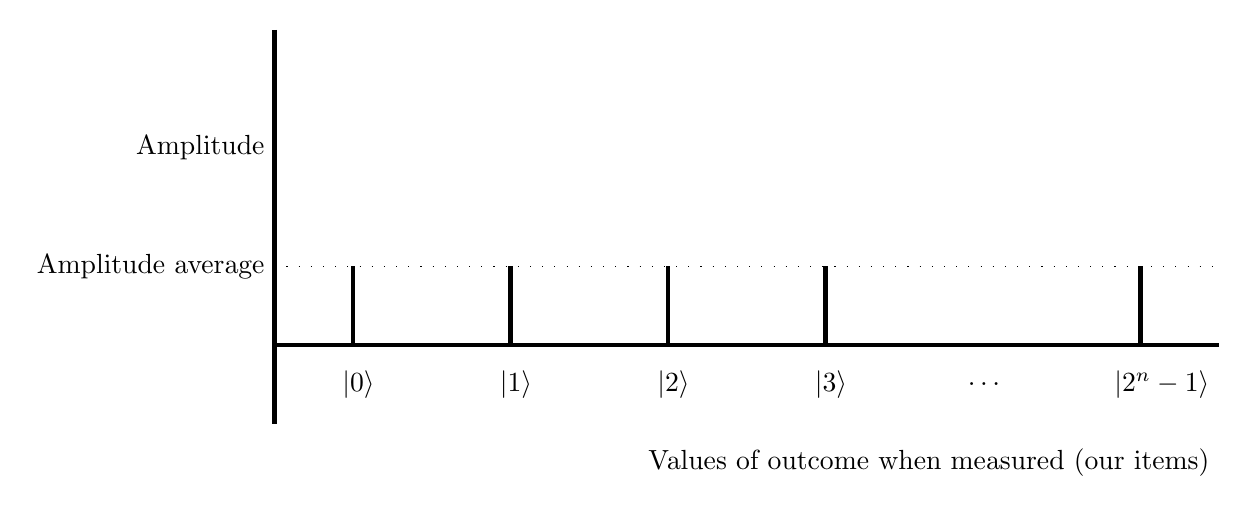
\begin{tikzpicture}
\draw[black, ultra thick] (0,0) -- (12,0);
\draw[black, ultra thick] (0,4) -- (0,-1);

\draw[black, ultra thick] (1,0) -- (1,1);
\draw[black] (1.4,-0.5) node[anchor=east]{$|0\rangle$};

\draw[black, ultra thick] (3,0) -- (3,1);
\draw[black] (3.4,-0.5) node[anchor=east]{$|1\rangle$};

\draw[black, ultra thick] (5,0) -- (5,1);
\draw[black] (5.4,-0.5) node[anchor=east]{$|2\rangle$};

\draw[black, ultra thick] (7,0) -- (7,1);
\draw[black] (7.4,-0.5) node[anchor=east]{$|3\rangle$};


\draw[black] (9.4,-0.5) node[anchor=east]{\dots};


\draw[black, loosely dotted] (0,1) -- (12,1);
\draw[black] (0,1) node[anchor=east]{Amplitude average};

\draw[black, ultra thick] (11,0) -- (11,1);
\draw[black] (12,-0.5) node[anchor=east]{$|2^{n} -1\rangle$};




\draw[black] (0,2.5) node[anchor=east]{Amplitude};
\draw[black] (12,-1.5) node[anchor=east]{Values of outcome when measured (our items)};
\end{tikzpicture}
\caption{Initial superposition of all items} \label{state_pref_graph}
\end{figure}
\end{center}

We represented the numbers in the kets in decimal format, but we refer to them as they would be in binary, this brings little bit of ambiguity because $|0\rangle$ in our diagram can represent the state $|00\rangle$ or $|000\rangle$, but from context it should be clear (in the following parts this will not be discussed, and the reader should be aware). 


\subsection{Applying oracle}
In this part of the algorithm, we point out correct solutions from our database. This can be done by performing a sequence of gates, which switches the amplitude of the correct solution to negative. Remember that we were precisely talking about not absolutely unifying the amplitude and probability in discussion about eq. \ref{one_qubit_}. Performing an oracle operation does not change the probability of measuring the correct result, it only changes the amplitude on the correct result. Oracle will be defined as a function $\mathfrak{O}$, which tells us whether $i$ in the combination \ref{mlti_qubit_state_chapter_2} is a solution or not. More formally, let $\mathfrak{O}:\{0,1\}^n \rightarrow \{0,1\}$, $\mathfrak{O}(\chi)=1$, if $|\chi\rangle$ is a solution, $\mathfrak{O}(\chi)=0$ otherwise. Then the matrix representation has the following pattern:

\begin{equation}
O = 
    \begin{bmatrix}
        -1^{\mathfrak{O}(|0\rangle)} & 0 & 0 & \cdots  & 0 & 0\\ 
        0 & -1^{\mathfrak{O}(|1\rangle)} & 0 & \cdots  & 0 & 0\\
        0 & 0 & -1^{\mathfrak{O}(|2\rangle)} & \cdots  & 0 & 0 \\
        \vdots & \vdots & \vdots & \ddots & \vdots & \vdots \\
        0 & 0 & 0 & \cdots  & -1^{\mathfrak{O}(|n-2\rangle)} & 0 \\
        0 & 0 & 0 & \cdots  & 0 & -1^{\mathfrak{O}(|n-1\rangle)} \\

    \end{bmatrix}.
\end{equation}

We will show that $O$ is unitary. For $O$ to be unitary it would have to mean:

\begin{equation}
    O \cdot \overline{O}^T =I.
\end{equation}
It is simple to see, that there is no imaginary number and transposing diagonal matrix will leave all the elements on the same place. The question now becomes if 

\begin{equation}
    O = O^{-1}.
\end{equation}

This, again, from simple observation is true, because the element on position $o_{j,j}$ can be 1 or -1. If it is 1, then, after multiplying it stays the same; if it is -1, then multiplying changes the value of $o_{j,j}$ to 1, therefore $O = O^{-1}$.

For a simple example, let $|0\rangle$ be the solution. So our diagram then changes as follows. In our diagram, it will be displayed as a visualisation of $|0\rangle$ as magenta instead of black.

\begin{center}
\begin{figure}[h]
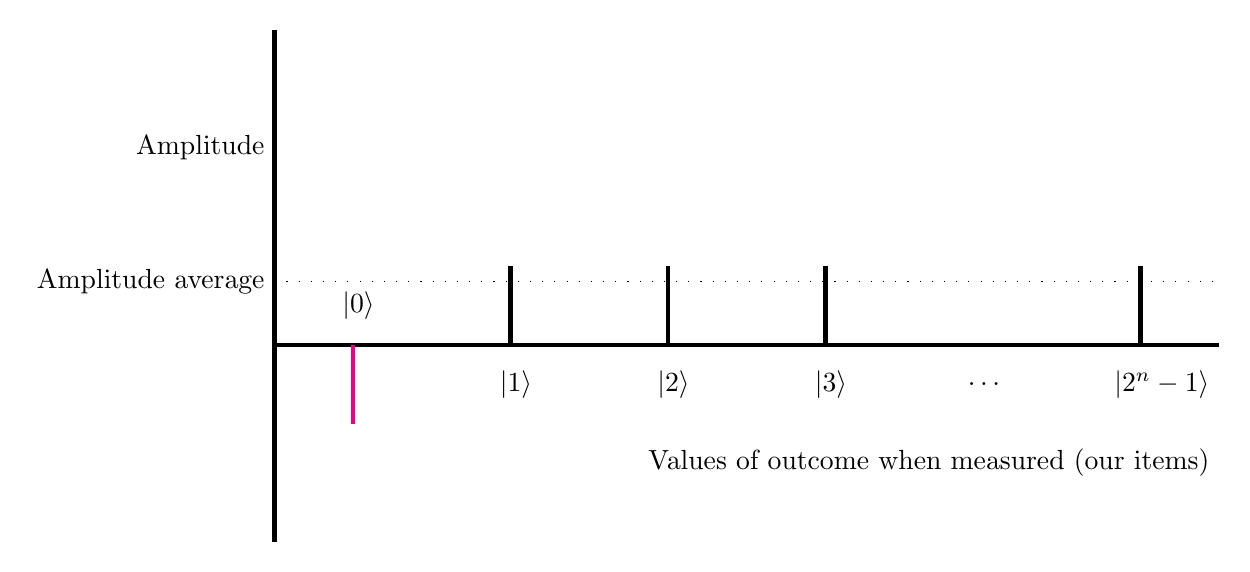
\begin{tikzpicture}
\draw[black, ultra thick] (0,0) -- (12,0);
\draw[black, ultra thick] (0,4) -- (0,-2.5);

\draw[magenta, ultra thick] (1,0) -- (1,-1);
\draw[black] (1.4,0.5) node[anchor=east]{$|0\rangle$};

\draw[black, ultra thick] (3,0) -- (3,1);
\draw[black] (3.4,-0.5) node[anchor=east]{$|1\rangle$};

\draw[black, ultra thick] (5,0) -- (5,1);
\draw[black] (5.4,-0.5) node[anchor=east]{$|2\rangle$};

\draw[black, ultra thick] (7,0) -- (7,1);
\draw[black] (7.4,-0.5) node[anchor=east]{$|3\rangle$};


\draw[black] (9.4,-0.5) node[anchor=east]{\dots};


\draw[black, loosely dotted] (0,0.8) -- (12,0.8);
\draw[black] (0,0.8) node[anchor=east]{Amplitude average};

\draw[black, ultra thick] (11,0) -- (11,1);
\draw[black] (12,-0.5) node[anchor=east]{$|2^{n} -1\rangle$};




\draw[black] (0,2.5) node[anchor=east]{Amplitude};
\draw[black] (12,-1.5) node[anchor=east]{Values of outcome when measured (our items)};
\end{tikzpicture}
\caption{Applying oracle} 
\end{figure}
\end{center}


We also see that the average amplitude has lowered because of the amplitude change of our result to a negative value instead of a positive. 
\newpage
\subsection{Applying diffuser} \label{TeoreticalDiffuser}
Now we rotate about the mean with the selected item, which has a negative amplitude. This results in something called amplitude amplification, where the selected item has a higher probability of being measured. The matrix representation is given by \begin{equation}
    D = 2 |\psi_{INIT} \rangle\langle \psi_{INIT} | - I;     |\psi_{INIT}\rangle = \sum_{i=0}^{2^n-1} \frac{|i\rangle }{\sqrt{2^n}}.
\end{equation}where $\psi_{INIT}$ is state of the quantum register after the state preparation. The diffuser $D$ can be expressed as following matrix:

\begin{equation}
D = 
    \begin{bmatrix}
        \frac{2}{2^n}-1 & \frac{2}{2^n} & \frac{2}{2^n} & \cdots  & \frac{2}{2^n} & \frac{2}{2^n}\\ 
        \frac{2}{2^n} & \frac{2}{2^n}-1 & \frac{2}{2^n} & \cdots  & \frac{2}{2^n} & \frac{2}{2^n}\\
        \frac{2}{2^n} & \frac{2}{2^n} & \frac{2}{2^n}-1 & \cdots  & \frac{2}{2^n} & \frac{2}{2^n} \\
        \vdots & \vdots & \vdots & \ddots & \vdots & \vdots \\
        \frac{2}{2^n} & \frac{2}{2^n} & \frac{2}{2^n} & \cdots  & \frac{2}{2^n}-1 & \frac{2}{2^n} \\
        \frac{2}{2^n} & \frac{2}{2^n} & \frac{2}{2^n} & \cdots  & \frac{2}{2^n} & \frac{2}{2^n} -1 \\

    \end{bmatrix}.
\end{equation}


\begin{center}
\begin{figure}
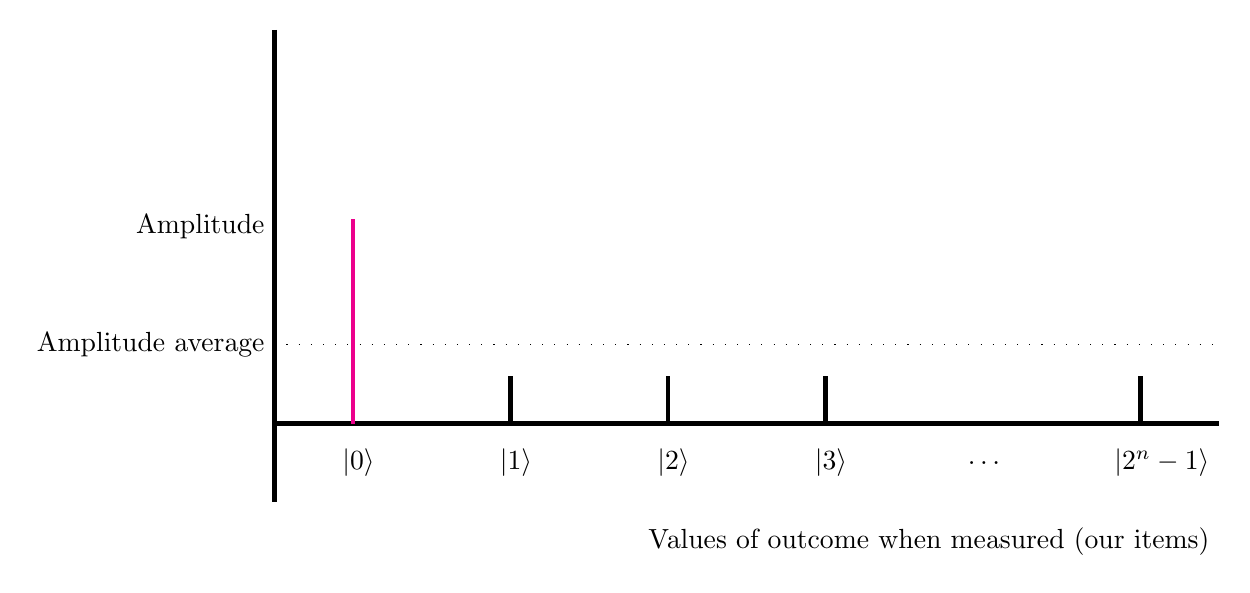
\begin{tikzpicture}
\draw[black, ultra thick] (0,0) -- (12,0);
\draw[black, ultra thick] (0,5) -- (0,-1);

\draw[magenta, ultra thick] (1,0) -- (1,2.6);
\draw[black] (1.4,-0.5) node[anchor=east]{$|0\rangle$};

\draw[black, ultra thick] (3,0) -- (3,0.6);
\draw[black] (3.4,-0.5) node[anchor=east]{$|1\rangle$};

\draw[black, ultra thick] (5,0) -- (5,0.6);
\draw[black] (5.4,-0.5) node[anchor=east]{$|2\rangle$};

\draw[black, ultra thick] (7,0) -- (7,0.6);
\draw[black] (7.4,-0.5) node[anchor=east]{$|3\rangle$};


\draw[black] (9.4,-0.5) node[anchor=east]{\dots};


\draw[black, loosely dotted] (0,1) -- (12,1);
\draw[black] (0,1) node[anchor=east]{Amplitude average};

\draw[black, ultra thick] (11,0) -- (11,0.6);
\draw[black] (12,-0.5) node[anchor=east]{$|2^{n} -1\rangle$};




\draw[black] (0,2.5) node[anchor=east]{Amplitude};
\draw[black] (12,-1.5) node[anchor=east]{Values of outcome when measured (our items)};
\end{tikzpicture}
\caption{Diffuser apply} 
\end{figure}
\end{center}
\newpage
\subsection{Further iterations description}
With the basic concept described, we can perform another repetition of applying the oracle and the diffuser to our quantum register.

Oracle apply:
\begin{center}
\begin{figure}[h]
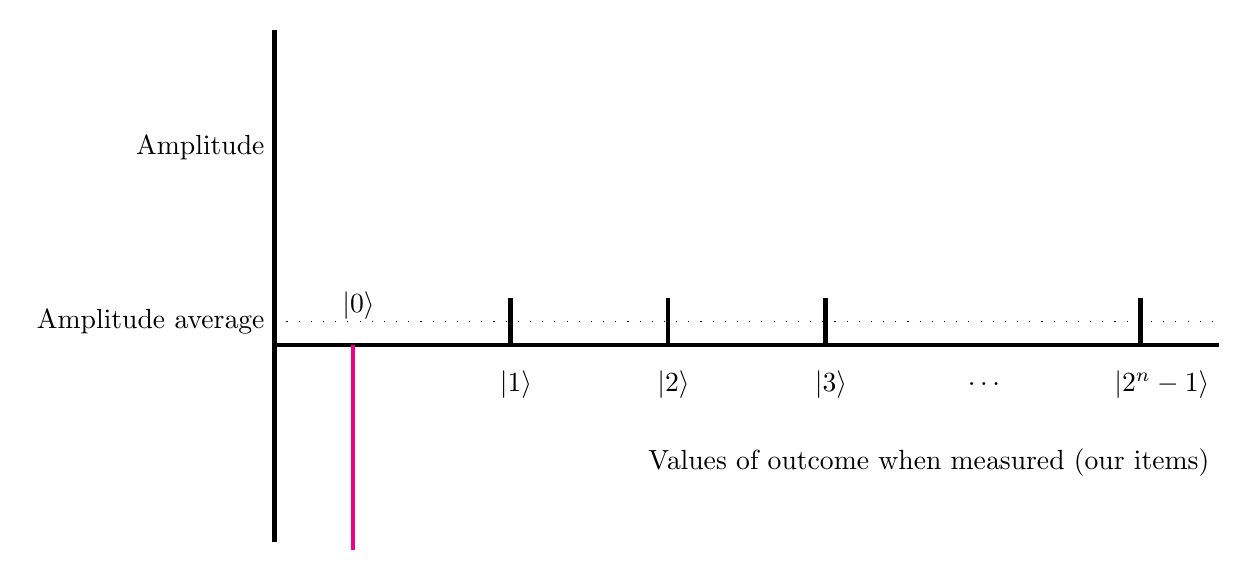
\begin{tikzpicture}
\draw[black, ultra thick] (0,0) -- (12,0);
\draw[black, ultra thick] (0,4) -- (0,-2.5);

\draw[magenta, ultra thick] (1,0) -- (1,-2.6);
\draw[black] (1.4,0.5) node[anchor=east]{$|0\rangle$};

\draw[black, ultra thick] (3,0) -- (3,0.6);
\draw[black] (3.4,-0.5) node[anchor=east]{$|1\rangle$};

\draw[black, ultra thick] (5,0) -- (5,0.6);
\draw[black] (5.4,-0.5) node[anchor=east]{$|2\rangle$};

\draw[black, ultra thick] (7,0) -- (7,0.6);
\draw[black] (7.4,-0.5) node[anchor=east]{$|3\rangle$};


\draw[black] (9.4,-0.5) node[anchor=east]{\dots};


\draw[black, loosely dotted] (0,0.3) -- (12,0.3);
\draw[black] (0,0.3) node[anchor=east]{Amplitude average};

\draw[black, ultra thick] (11,0) -- (11,0.6);
\draw[black] (12,-0.5) node[anchor=east]{$|2^{n} -1\rangle$};




\draw[black] (0,2.5) node[anchor=east]{Amplitude};
\draw[black] (12,-1.5) node[anchor=east]{Values of outcome when measured (our items)};
\end{tikzpicture}
\caption{Second apply of the oracle} 
\end{figure}
\end{center}

Diffuser apply:
\begin{center}
\begin{figure}[h]
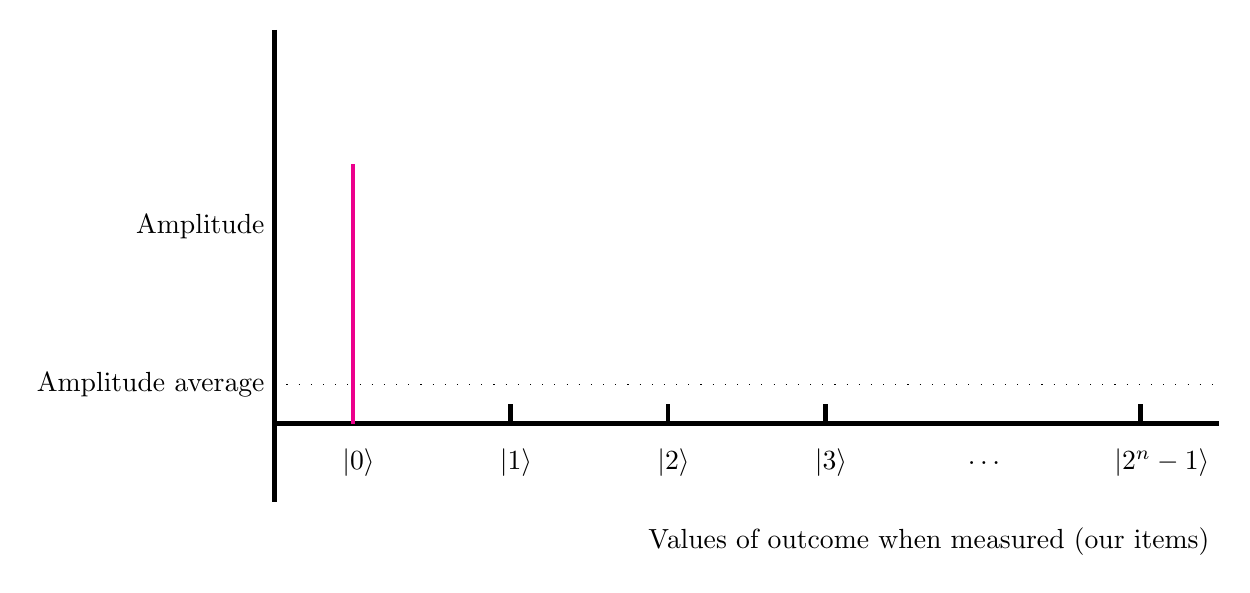
\begin{tikzpicture}
\draw[black, ultra thick] (0,0) -- (12,0);
\draw[black, ultra thick] (0,5) -- (0,-1);

\draw[magenta, ultra thick] (1,0) -- (1,3.3);
\draw[black] (1.4,-0.5) node[anchor=east]{$|0\rangle$};

\draw[black, ultra thick] (3,0) -- (3,0.25);
\draw[black] (3.4,-0.5) node[anchor=east]{$|1\rangle$};

\draw[black, ultra thick] (5,0) -- (5,0.25);
\draw[black] (5.4,-0.5) node[anchor=east]{$|2\rangle$};

\draw[black, ultra thick] (7,0) -- (7,0.25);
\draw[black] (7.4,-0.5) node[anchor=east]{$|3\rangle$};


\draw[black] (9.4,-0.5) node[anchor=east]{\dots};


\draw[black, loosely dotted] (0,0.5) -- (12,0.5);
\draw[black] (0,0.5) node[anchor=east]{Amplitude average};

\draw[black, ultra thick] (11,0) -- (11,0.25);
\draw[black] (12,-0.5) node[anchor=east]{$|2^{n} -1\rangle$};


            

\draw[black] (0,2.5) node[anchor=east]{Amplitude};
\draw[black] (12,-1.5) node[anchor=east]{Values of outcome when measured (our items)};
\end{tikzpicture}
\caption{Second apply of the diffuser}
\end{figure}
\end{center}

We see that the second apply of the oracle and the diffuser had a much smaller impact on our quantum register. All this time we had an amplitude average positive value, performing one more application of the oracle and the diffuser would result in lowering the chance of the solution being measured because the oracle would set the amplitude average to a negative value; thus, the rotation about the mean would have an unwanted effect on our register.

It is a good idea to show the combined matrix of diffuser and oracle, as it shows more in debt how the algorithm works. We will show this for one solution. For demonstrational purpouses, we assume that $|0\rangle$ is the solution, as we have shown in our diagrams.

\begin{equation}
    \iota = DO =
    \begin{bmatrix}
        \frac{2}{2^n}-1 & \frac{2}{2^n} & \frac{2}{2^n} & \cdots  & \frac{2}{2^n} & \frac{2}{2^n}\\ 
        \frac{2}{2^n} & \frac{2}{2^n}-1 & \frac{2}{2^n} & \cdots  & \frac{2}{2^n} & \frac{2}{2^n}\\
        \frac{2}{2^n} & \frac{2}{2^n} & \frac{2}{2^n}-1 & \cdots  & \frac{2}{2^n} & \frac{2}{2^n} \\
        \vdots & \vdots & \vdots & \ddots & \vdots & \vdots \\
        \frac{2}{2^n} & \frac{2}{2^n} & \frac{2}{2^n} & \cdots  & \frac{2}{2^n}-1 & \frac{2}{2^n} \\
        \frac{2}{2^n} & \frac{2}{2^n} & \frac{2}{2^n} & \cdots  & \frac{2}{2^n} & \frac{2}{2^n} -1 \\
    \end{bmatrix}\cdot
    \begin{bmatrix}
        -1 & 0 & 0 & \cdots  & 0 & 0\\ 
        0 & 1 & 0 & \cdots  & 0 & 0\\
        0 & 0 & 1 & \cdots  & 0 & 0 \\
        \vdots & \vdots & \vdots & \ddots & \vdots & \vdots \\
        0 & 0 & 0 & \cdots  & 1 & 0 \\
        0 & 0 & 0 & \cdots  & 0 & 1 \\

    \end{bmatrix}.
\end{equation}

\begin{equation} \label{one_grover_iteration_matrix}
    \iota =
    \begin{bmatrix}
        
        1-\frac{2}{2^n} & \frac{2}{2^n} & \frac{2}{2^n} & \cdots  & \frac{2}{2^n} & \frac{2}{2^n}\\ 
        -\frac{2}{2^n} & \frac{2}{2^n}-1 & \frac{2}{2^n} & \cdots  & \frac{2}{2^n} & \frac{2}{2^n}\\
        -\frac{2}{2^n} & \frac{2}{2^n} & \frac{2}{2^n}-1 & \cdots  & \frac{2}{2^n} & \frac{2}{2^n} \\
        \vdots & \vdots & \vdots & \ddots & \vdots & \vdots \\
        -\frac{2}{2^n} & \frac{2}{2^n} & \frac{2}{2^n} & \cdots  & \frac{2}{2^n}-1 & \frac{2}{2^n} \\
        -\frac{2}{2^n} & \frac{2}{2^n} & \frac{2}{2^n} & \cdots  & \frac{2}{2^n} & \frac{2}{2^n} -1 \\ 
   
    \end{bmatrix}.
\end{equation}

\section{Algorithm analysis and complexity description}

\subsection{Recurrence equations for the algorithm} \label{Recurrence_eq_grover}
Suppose that we have done the first step, the state preparation, and that currently our quantum register is 

\begin{equation}
    |\psi_{INIT}\rangle =  \sum_{i=0}^{2^n-1} \frac{|i\rangle }{\sqrt{N}} =\sum_{i=0}^{2^n-1}\frac{|i\rangle }{\sqrt{2^n}}.
\end{equation}

First we show a system of linear recurrence equations with a parameter as a potential way to derive optimal number of iterations for one solution.

Say we have $\Lambda$, $\Theta$ $\in {\rm I\!R}$, where $\Lambda$ is the amplitude of the correct solution and $\Theta$ is the amplitude of the bad solution. We can continue with the description with eq. \ref{one_grover_iteration_matrix}. We have assumed that $|0\rangle$ is the solution; this means that the first row in the matrix represents an increase or decrease in $\Lambda$. As the algorithm is iterative, we can describe it with a sequence. $\Lambda$ in the $k+1$th step will be equal to

\begin{equation} \label{lambda_increment_first}
    \Lambda_{k+1} = (1-\frac{2}{2^n})\Lambda_k + (2^n -1)\frac{2}{2^n}\Theta_k,
\end{equation}
which can be rewritten as
\begin{equation}
    \Lambda_{k+1}= (1-\frac{2}{2^n})\Lambda_k + (2 - \frac{2}{2^n})\Theta_k.
\end{equation}
Similarly $\Theta$ in the $k+1$th step will be
\begin{equation}
    \Theta_{k+1} = -\frac{2}{2^n}\Lambda_k +(\frac{2}{2^n}-1)\Theta_k +(2^n -2)\frac{2}{2^n}\Theta_k,
\end{equation}
rewriting it as
    \begin{equation}
    \Theta_{k+1} = -\frac{2}{2^n}\Lambda_k +(\frac{2}{2^n}-1 +2 -\frac{4}{2^n})\Theta_k,
    \end{equation}
after simplification,
\begin{equation}
    \Theta_{k+1} = -\frac{2}{2^n}\Lambda_k +(1 -\frac{2}{2^n})\Theta_k.
\end{equation}

Suppose that we have $m$ solutions and $n$ qubits. Then the solution will be slightly different. In eq. \ref{one_grover_iteration_matrix} it would lead to $m$ rows being multiplied by minus one in addition to just one solution. 

\begin{equation} 
    \Lambda_{k+1} = (1-\frac{2}{2^n})\Lambda_k - (m-1)\frac{2}{2^n}\Lambda_k + (2^n - m)\frac{2}{2^n}\Theta_k,
\end{equation}

\begin{equation} 
    \Lambda_{k+1} = (1-\frac{2}{2^n} - \frac{2m}{2^n} +\frac{2}{2^n})\frac{2}{2^n}\Lambda_k + (2^n - m)\frac{2}{2^n}\Theta_k,
\end{equation}

\begin{equation} \label{multi_solution_lambda_last}
    \Lambda_{k+1} = (1 - \frac{2m}{2^n})\Lambda_k + (2^n - m)\frac{2}{2^n}\Theta_k,
\end{equation}

we see that if $m=1$ we get the eq. \ref{lambda_increment_first}. Let us do the same thing for $\Theta$

\begin{equation} 
    \Theta_{k+1} = -\frac{2}{2^n}m\Lambda_k +(\frac{2}{2^n}-1)\Theta_k +(2^n - m -1)\frac{2}{2^n}\Theta_k,
\end{equation}

\begin{equation} 
    \Theta_{k+1} = -\frac{2}{2^n}m\Lambda_k +(\frac{2}{2^n}-1 + 2 - \frac{2m}{2^n} -\frac{2}{2^n})\Theta_k,
\end{equation}

\begin{equation} \label{multi_solution_theta_last}
    \Theta_{k+1} = -\frac{2}{2^n}m\Lambda_k +(1 -\frac{2m}{2^n})\Theta_k,
\end{equation}


We shall discuss eq. \ref{multi_solution_lambda_last} and eq. \ref{multi_solution_theta_last}. $\Lambda_k$ will have the highest value when $\Delta_{k}=\Lambda_{k+1}-\Lambda_k$ reaches the first negative value.
\subsection{Geometrical analysis}

From subsection \ref{Recurrence_eq_grover} we can see that the number of iterations depends on the number of solutions and on the number of qubits used. We will start with one solution and $n$ qubits, we will approach it from one of the perspectives shown in \cite{qc_grover} and \cite{qc_grover_microsoft}.

We begin by constructing a plane $\mathbb{G}$ with two orthogonal states $|\tau\rangle$ and $|\upsilon\rangle$ and our initial state $|\psi_{INIT} \rangle$ and an angle $\frac{\phi}{2}$, which is the angle between $|\psi_{INIT} \rangle$ and $|\upsilon\rangle.$ Let us also define an angle $\zeta$, which is the angle between $|\psi\rangle$ and $|\upsilon\rangle$, after initialization it is same as $\frac{\phi}{2}$.We can express any state in this plane with
\begin{equation} \label{basic_quantum_state_geom}
    |\psi\rangle = \alpha |\tau \rangle  + \beta|\upsilon\rangle.
\end{equation}

Difference between $\alpha$ and $\beta$ from eq. \ref{basic_quantum_state} and from eq. \ref{basic_quantum_state_geom} is that in eq. \ref{basic_quantum_state_geom} $\alpha$, $\beta \in{\rm I\!R}$, while in eq. \ref{basic_quantum_state} $\alpha$, $\beta \in \mathbb{C}$.

With substitution to eq. \ref{basic_quantum_state_geom} we can rewrite it as
\begin{equation}
    |\psi_{INIT}\rangle = sin\Bigl(\frac{\phi}{2}\Bigr)|\tau \rangle  + cos\Bigl(\frac{\phi}{2}\Bigr)|\upsilon\rangle,
\end{equation}

\begin{figure}[h]
\begin{center}
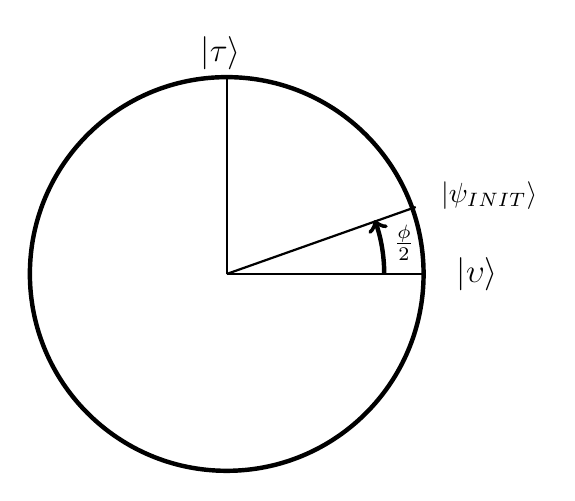
\begin{tikzpicture}
\draw[ultra thick](0,0) circle (2.5);

\draw[black,thick] (0,0) -- (2.5,0);
\draw[black] (0.3,2.8) node[anchor=east,font=\large]{$|\tau\rangle$};

\draw[black, thick] (0,0) -- (0,2.5);
\draw[black] (2.8,0) node[anchor=west,font=\large]{$|\upsilon\rangle$};

\draw[black, thick] (0,0) -- (2.4,0.85);
\draw[black] (2.6,1) node[anchor=west,font=\normalsize]{$|\psi_{INIT}\rangle$};

\draw[ultra thick, ->] (2,0) arc (0:20:2);
\draw[black] (2,0.4) node[anchor=west,font=\normalsize]{$\frac{\phi}{2}$};


\end{tikzpicture}
\caption{Preparation} \label{GA_prep}
\end{center}
\end{figure}

Let's introduce an oracle and its effect on $|\psi_{INIT}\rangle$. Say, we have $|\omega\rangle$ and $|\omega^{\perp}\rangle$, which is orthogonal to $|\omega\rangle$ in $\mathbb{G}$. Let us have $\Hat{\psi}=\Hat{\alpha}|\omega\rangle + \Hat{\beta}|\omega^{\perp}\rangle$. This is satisfied by
\begin{equation}
    |\omega\rangle = sin\Bigl(\Hat{\phi}\Bigr)|\tau \rangle  + cos\Bigl(\Hat{\phi}\Bigr)|\upsilon\rangle
\end{equation}
and
\begin{equation}
    |\omega^{\perp}\rangle = cos\Bigl(\Hat{\phi}\Bigr)|\tau \rangle  -sin\Bigl(\Hat{\phi}\Bigr)|\upsilon\rangle
\end{equation}
This can be shown easily by showing
\begin{equation}
    \langle \omega^{\perp}|\omega\rangle = 0.
\end{equation}
\begin{equation}
     \biggl(cos\Bigl(\Hat{\phi}\Bigr)\langle\tau |  -sin\Bigl(\Hat{\phi}\Bigr)\langle \upsilon|\biggl)\biggl(sin\Bigl(\Hat{\phi}\Bigr)|\tau \rangle  + cos\Bigl(\Hat{\phi}\Bigr)|\upsilon\rangle\biggl),
\end{equation}

\begin{equation}
     cos^2\Bigl(\Hat{\phi}\Bigr)\langle\tau | \upsilon \rangle -sin^2\Bigl(\Hat{\phi}\Bigr)\langle \upsilon|\tau \rangle + sin\Bigl(\Hat{\phi}\Bigr)cos\Bigl(\Hat{\phi}\Bigr)\langle\tau|\tau \rangle  - sin\Bigl(\Hat{\phi}\Bigr)cos\Bigl(\Hat{\phi}\Bigr)\langle\upsilon|\upsilon\rangle,
\end{equation}
$|\upsilon\rangle$ and $|\tau\rangle$ are orthogonal,
\begin{equation}
sin\Bigl(\Hat{\phi}\Bigr)cos\Bigl(\Hat{\phi}\Bigr)\langle\tau|\tau \rangle  - sin\Bigl(\Hat{\phi}\Bigr)cos\Bigl(\Hat{\phi}\Bigr)\langle\upsilon|\upsilon\rangle,
\end{equation}
$\langle\psi|\psi\rangle=1$ for any state $|\psi\rangle$,
\begin{equation}
    sin\Bigl(\Hat{\phi}\Bigr)cos\Bigl(\Hat{\phi}\Bigr)  - sin\Bigl(\Hat{\phi}\Bigr)cos\Bigl(\Hat{\phi}\Bigr) =0.
\end{equation}
Oracle leads to rotation around $|\upsilon\rangle$ in fig. \ref{GA_prep}.


\begin{figure}[ht]
\begin{center}
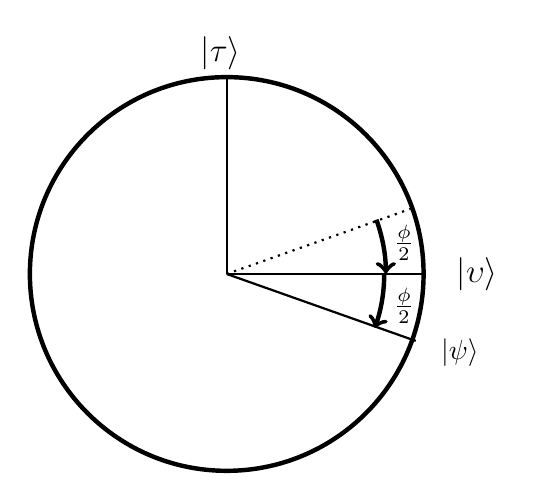
\begin{tikzpicture}
\draw[ultra thick](0,0) circle (2.5);

\draw[black,thick] (0,0) -- (2.5,0);
\draw[black] (0.3,2.8) node[anchor=east,font=\large]{$|\tau\rangle$};

\draw[black, thick] (0,0) -- (0,2.5);
\draw[black] (2.8,0) node[anchor=west,font=\large]{$|\upsilon\rangle$};

\draw[black, thick,dotted] (0,0) -- (2.4,0.85);


\draw[ultra thick, ->] (1.9,0.69) arc (20:0:2);
\draw[black] (2,0.4) node[anchor=west,font=\normalsize]{$\frac{\phi}{2}$};

\draw[ultra thick, ->] (2,0) arc (0:-20:2);
\draw[black] (2,-0.4) node[anchor=west,font=\normalsize]{$\frac{\phi}{2}$};

\draw[black, thick] (0,0) -- (2.4,-0.85);
\draw[black] (2.6,-1) node[anchor=west,font=\normalsize]{$|\psi\rangle$};

\end{tikzpicture}
\caption{Oracle rotation} \label{GA_oracle_geom}
\end{center}
\end{figure}


\begin{equation}
    |\psi\rangle = O|\psi_{INIT}\rangle = -sin\Bigl(\frac{\phi}{2}\Bigr)|\tau \rangle  + cos\Bigl(\frac{\phi}{2}\Bigr)|\upsilon\rangle,
\end{equation}
It is worth pointing out, that the angle $\zeta$ changes to $\frac{-\theta}{2}$, but the functions  have the properties of $sin(-x)=-sin(x)$ and $cos(x)=cos(-x)$.

%From observation we see that $|\psi_{INIT}\rangle\perp O|\psi_{INIT}\rangle$ in $|\omega\rangle$ and $|\omega^{\perp}\rangle$ basis as we defined it as orthogonal.

The iteration ends with the application of the diffuser.  Let us define the diffuser as $D = 2|\omega\rangle\langle\ \omega|-I$, then the diffuser has the following effect.
\begin{equation}
    D\Hat{\psi}=D(\Hat{\alpha}|\omega\rangle + \Hat{\beta}|\omega^{\perp}\rangle),
\end{equation}
after expanding D,
\begin{equation}
    D\Hat{\psi}=(2|\omega\rangle\langle\omega|-I)(\Hat{\alpha}|\omega\rangle + \Hat{\beta}|\omega^{\perp}\rangle),
\end{equation}

\begin{equation}
    D\Hat{\psi}=(2\Hat{\alpha}|\omega\rangle\langle\omega|\omega\rangle-\Hat{\alpha}|\omega\rangle) + 2\Hat{\beta}|\omega\rangle\langle\omega|\omega^{\perp}\rangle - \Hat{\beta}|\omega^{\perp}\rangle,
\end{equation}
$\langle\omega|\omega\rangle=1$ and $\langle\omega|\omega^{\perp}\rangle=0$ leads to
\begin{equation}
    D\Hat{\psi}=\Hat{\alpha}|\omega\rangle - \Hat{\beta}|\omega^{\perp}\rangle.
\end{equation}

In our plane $\mathbb{G}$ this leads to the following reflection, where we choose $\Hat{\phi}=\frac{\phi}{2}$.

\begin{figure}[h]
\begin{center}
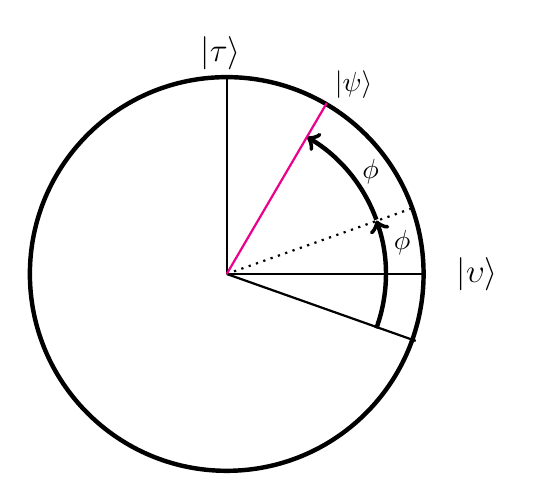
\begin{tikzpicture}
\draw[ultra thick](0,0) circle (2.5);

\draw[black,thick] (0,0) -- (2.5,0);
\draw[black] (0.3,2.8) node[anchor=east,font=\large]{$|\tau\rangle$};

\draw[black, thick] (0,0) -- (0,2.5);
\draw[black] (2.8,0) node[anchor=west,font=\large]{$|\upsilon\rangle$};

\draw[black, thick,dotted] (0,0) -- (2.4,0.85);


\draw[ultra thick, ->] (1.9,-0.69) arc (-20:20:2);
\draw[black] (2,0.4) node[anchor=west,font=\normalsize]{$\phi$};

\draw[ultra thick, ->] (1.9,0.69) arc (20:60:2);
\draw[black] (1.6,1.3) node[anchor=west,font=\normalsize]{$\phi$};

\draw[black, thick] (0,0) -- (2.4,-0.85);

\draw[magenta, thick] (0,0) -- (1.27,2.17);
\draw[black] (1.25,2.4) node[anchor=west,font=\normalsize]{$|\psi\rangle$};

\end{tikzpicture}
\caption{Diffuser reflection} \label{GA_diffuser_geom}
\end{center}
\end{figure}
After applying the oracle the angle stayed the same as we see in fig. \ref{GA_oracle_geom}, the only change was it changed to negative value. The difference was made with the diffuser, since the diffuser had reflection about $|\psi_{INIT}\rangle$, so one iteration $\iota$ of the algorithm increases $\zeta$ by the angle $\phi$ as seen in the figures.

After the iteration, the angle increases, this leads to 
\begin{equation}
    |\psi\rangle = sin\Bigl(\frac{3\phi}{2}\Bigr)|\tau \rangle  + cos\Bigl(\frac{3\phi}{2}\Bigr)|\upsilon\rangle,
\end{equation}
so after $k$ iterations the formula looks like following:
\begin{equation}
        |\psi\rangle = sin\Bigl(\phi k+\frac{\phi}{2}\Bigr)|\tau \rangle  + cos\Bigl(\phi k+\frac{\phi}{2}\Bigr)|\upsilon\rangle,
\end{equation}
which can be rewritten as
\begin{equation}
        |\psi\rangle = sin \Bigl(\phi (k+\frac{1}{2})\Bigr)|\tau \rangle  + cos\Bigl(\phi (k+\frac{1}{2})\Bigr)|\upsilon\rangle,
\end{equation}
so $\zeta = \phi (k+\frac{1}{2}).$

We can view $\tau$ as a solution to the problem and $ \upsilon $ not as a solution. As we are discussing a situation with one solution,
\begin{equation}
    |\psi_{INIT}\rangle=\sqrt{\frac{1}{2^n}}|\tau\rangle+\sqrt{1-\frac{1}{2^n}}|\upsilon\rangle.
\end{equation}
For small angles, we can estimate $\sqrt{\frac{1}{2^n}}=sin(\frac{\phi}{2})\approx\frac{\phi}{2}$.

We want to minimise the probability of measuring $|\upsilon\rangle$, which is given by $cos^2\Bigl(\phi (k+\frac{1}{2})\Bigr)$. This function has its first local minimum in $\frac{\pi}{2}$.

\begin{equation}
    \frac{\pi}{2} = \phi (k+\frac{1}{2}),
\end{equation}
using approximation for $\phi$,
\begin{equation}
    \frac{\pi}{2} = 2\sqrt{\frac{1}{2^n}} (k+\frac{1}{2}),
\end{equation}

\begin{equation}
    \frac{\pi}{2} = 2\sqrt{\frac{1}{2^n}} k+\sqrt{\frac{1}{2^n}},
\end{equation}
\begin{equation}
    \frac{\pi}{2}\sqrt{2^n} = 2k+1,
\end{equation}
\begin{equation}
    k=\frac{\pi}{4}\sqrt{2^n}-\frac{1}{2}.
\end{equation}
With taking $m$ solutions rather than one our approximation for $\frac{\phi}{2}$ would be $\sqrt{\frac{m}{2^n}}=sin(\frac{\phi}{2})\approx\frac{\phi}{2}$, leading to small change in solution.
\begin{equation} \label{optimal_iter}
    k=\frac{\pi}{4}\sqrt\frac{2^n}{m}-\frac{1}{2}.
\end{equation}

We have shown the optimal number of iterations with this geometrical approach.
